\section{Analysis} \label{sec:analysis}


% Pacman content research


\subsection{Pacman}
\subsubsection{AI behaviour argumentation (how they do it)}
\subsubsection{Technical details/mechanics/paramters}

\subsection{Player performance}
a. Identify pacman parameters to measure player performance. (from 4.B) Associate also with  previous research(other AI implementations in Pacman. What did they use to  identify “performance”?


b. Define “good” and “bad” performance based upon 5a. (assume that we use only win/lose conditions unless prior research has based performance indications upon other game parameter results)

c. Performance results. We identify “some” performance. Therefore we configure the following “alternation of ghost behavior” in “this” way.

\subsection{Genetic Algorithm(s)}

\subsubsection{Description}
Genetic algorithms was invented by John Holland in 1975 and is proposed as a heuristic method, which is a method to learn by itself based upon survival of the fittest, where it is described as a  search algorithm that uses mechanisms much like evolution to improve some solutions to a given problem. \cite[pp. 20]{Sivanandam2008}

The Genetic Algorithm start with a set of plausible solutions and by the use of genetic operator alterations like reproduction, crossovers and mutations \cite{Baltzer2014}, it develops a new set of better solutions compared to the previous. By repeating this process, a population will theoretically improve until a satisfying result is found to the given problem. \cite{BCS2013}

What is noteworthy about "satisfying results" is that we search for some better solution within a set of possible solutions, also referred to as search space. It is therefore not guaranteed to find some, if any, optimal solution to the problem but rather a solution which can be interpreted as acceptably good. \cite[pp. 20/21]{Sivanandam2008}


In genetic algorithms, populations and individuals covers the terminology of the solutions and searches thereof. A individual is to be considered a single solution to the problem and the population is the number of individuals involved. \cite[pp. 39]{Sivanandam2008} 



\subsubsection{Genetic Algorithm Components}

A Genetic Algorithm consists of at least five components as described by Baltzer, 2014 \cite{Baltzer2014}. These components can be considered to be the main components in any genetic algorithm.
\begin{itemize}
\item \textbf{Chromosome / gene representation}

A representation of a population and the subordinate content, being chromosomes and genes as seen on figure \ref{fig:gene}.
The genes functions as a string of some arbitrary length of data. A chromosome is a sequence of genes, whereof the combined chromosomes serves as the population. \cite[pp. 41]{Sivanandam2008} 

As mentioned above, each individual(chromosome) is a single solution to the problem at hand. The chromosomes can be considered to be \enquote{a point in the search space of candidate solutions} \cite[pp. 7]{Melanie1990} Melanie, 1990.
	

\begin{figure}[!h]
\centering
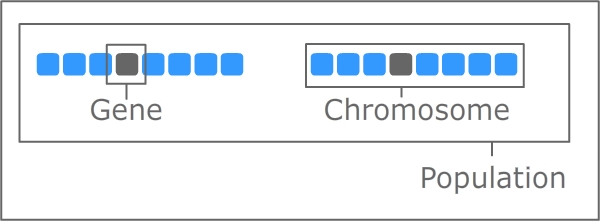
\includegraphics[scale=1.0]{gene_chromosomes.jpg}
\caption{gene, chromosomes and population description}
\label{fig:gene}
\end{figure}

\item \textbf{Initialisation of the population}

A population is a collection of individuals(chromosomes).  

An initial population must be created as a starting point for the algorithm. This representation of a population is chosen randomly, as there might be no prior evident solutions. Dependent on the stated problem at hand, the initialization of populations might also be carried out with some good solutions to the problem. However in most cases, the initial population is chosen at random. \cite[pp. 41/42]{Sivanandam2008}



\item \textbf{evaluation function(fitness)}

In order to improve further generations, the fitness of each chromosome in the current population must be evaluated. The genetic algorithm does so by the use of a fitness function, which assign some score(fitness) to each of the chromosomes within a specific population.
In general manners, the fitness of a given chromosome is dependant on how successively the given chromosome solved the designated problem, and is conveyed through a range of values. The better the solution, the higher the fitness score \cite[pp. 8]{Melanie1990}

how "good" the solution is, is the whole purpose of the fitness function to identify. the fitness function perform some evaluation of the acquired results and then assigns specific fitness score to that solution. How the fitness function performs the evaluation of solution is dependent on the problem itself. There are no single solutions as to how the fitness function is to be developed, but can be really be anything, that successively covers the plausible methods of evaluating the solutions. \cite[pp. 31]{Sivanandam2008}




\item \textbf{Genetic operators altering chromosomes(reproduction/selection, crossover and mutation.}


Genetic operators in some of the more simple Genetic Algorithms are reproduction/selection, crossover and mutation. Melanie, 1990. \cite{Melanie1990}

\textbf{reproduction/selection:} \enquote{This operator selects chromosomes in the population for reproduction. The fitter the chromosome, the more times it is likely to be selected to reproduce.} \cite[pp. 8]{Melanie1990}
The idea behind this operator is that preferences are given to the better chromosomes in the population, which is then passed on to the next generation. This is based upon the fitness score.

Within the selection operator, several selection methods exists which defines how the actual selection of "best" individuals is to be conducted. 

Some of the selection methods are:
\begin{itemize}
\item Roulette Wheel Selection
\item Random Selection
\item Rank Selection
\item Tournament Selection
\item Boltzmann Selection
\item Stochastic Universal Sampling
\item Steady-State Selection
\item Elitism
\item Fitness Proportionate selection
\item Scaling Selection
\item Generation Selection
\item Hierachical Selection
\end{itemize}
The list is from Sivanandam, 2008 \cite[pp. 46-50]{Sivanandam2008} and Markzyk, 2004 \cite{Adam2004}.

The different selection methods will not be accounted for and described in this chapter, however the appropriate selection method will be accessed in the design chapter along with descriptive reasoning and method of application of the selected method(s), or combination of such.

\textbf{Crossover:} \enquote{This operator randomly chooses a locus and exchange the subsequences before and after that locus between two chromosomes to create two offspring.} \cite[pp. 8]{Melanie1990}

The crossover method takes two parent solutions(chromosomes) to create new individuals, by swapping genes between two of the potentially good solutions. There exists several crossover methods, which are:


\begin{itemize}
\item Single Point Crossover
\item Two Point Crossover
\item Multi-Point Crossover (N-Point crossover)
\item Uniform Crossover
\item Three Parent Crossover
\item Crossover with Reduced Surrogate
\item Shuffle Crossover
\item Precedence Preservative Crossover (PPX)
\item Ordered Crossover
\item Partially Matched Crossover (PMX)
\end{itemize}
The list is from Sivanandam, 2008 \cite[pp. 50-56]{Sivanandam2008}

Similarly with the list of selection operators, we will not account for the crossover operator methods, but will be accessed in the design chapter with similar procedures and content. 

Additionally with the crossover operator, we can describe the crossover probability.
The crossover probability is a parameter that describes the likelihood of crossover. It basically states how often that the crossover method will be performed.\cite[pp. 56]{Sivanandam2008}

The crossover probability determines how the new generation(offspring) is altered. If there is some crossover probability then the offspring will contain genes from both of the parent chromosomes. If there is no crossover probability then the offspring will be copies of the parent chromosomes. They will be exact copies, but does not mean that they are the same.


\textbf{Mutation:} \enquote{This operator randomly flips some of the bits in a chromosome.} \cite[pp. 8]{Melanie1990}

The mutation operator happens after the crossover operator. The mutation randomly alters the structure(ordering of the genes) within the chromosomes or randomly modifies it.
The mutation of the chromosomes can happen in the following manners, dependent on the kind of representation of genes; flipping, interchanging and reversing.\cite[pp. 57]{Sivanandam2008}

Flipping genes/values is simply alterations of some to other, and other to some which then indicates a child from that chromosome. Example can be that a gene(1) is converted to gene(0), and gene(0) is converted to gene(1).

Interchanging is randomly assigning two genes within a chromosome and then switch locations of the two genes.

Lastly, reversing is randomly choosing a gene within a chromosome and thereafter change the location of the gene with a gene next to it.

Much like crossover probability, there is also a mutation probability. It states how often parts of the chromosome will be mutated. If a mutation occurs, then the chromosome is changed, in some way as specified above. If the mutation probability is 0 percent, then no mutation occurs and if the mutation is at 100 percent, then the whole chromosome is changed in accordance with the type of mutation that is specified. The reason to implement mutation of the chromosomes is to ensure that the genetic algorithm does not fall into some local extremes.\cite[pp. 57]{Sivanandam2008}

\item \textbf{Parameters for population size and probabilities of genetic operators.}
\end{itemize}

The population size covers the amount of solutions(chromosomes) that is in the actual population in the search space. The actual size of the population does very much depend on the problem at hand.\cite[pp. 42]{Sivanandam2008}


Another important aspect is the actual probability of the mutation and crossover operations.
It is mentioned in the appropriate sections concerning mutation and crossover what happens in in the absence(0 percent) or fully enabled(100 percent), but does not account for the most efficient percentage of the two. It is however also dependent on the problem, so finding some specific value, or range of values to a percentage of the crossover or mutation probability will not be possible to define, before the actual problem is defined along with some indications of plausible solutions.

The alterations in the probability may or may not have positive effects on the new generations of populations.

Marek, 1998\cite{Marek1998}  describes some recommendations based upon emprirical studies which plausible can be used as a reference point, but can be considered to be general and not necessarily the most optimal configurations, so alterations and adjustments must be conducted to account for the specific problem at hand.

the general recommendations are described as followed:
\begin{itemize}
\item Crossover rate: 80-95 percent.

It is however mentioned that occurrences of crossover probabilities of 60 percent was optimal in some undefined problem scenarios.
\item Mutation rate: 0.5-1.0 percent

The mutation rate are described as being optimal when very low.
\item population size

It is described that population size very much depend on encoding and size of the chromosomes. a population size of 20-30 is stated as good, but other examples of 50-100 are also accounted for as a good population size.
\end{itemize}

\subsubsection{Genetic algorithm procedure}

Now that the general usage, definition and components has been described, a short general description of the procedure as to implementation and functionality of a general algorithm can be defined.

Each iteration of the genetic algorithm process is defined as a generation. The entire set of generations is defined as a run. \cite[pp. 9]{Melanie1990}

A general genetic algorithm is here defined algorithmically by Malhotra et.al, 2011 \cite[pp. 40]{Rahul2011}
\enquote{
\begin{description}
\item[Start:] Generate population of chromosomes.
\item[Fitness:] Evaluate fitness score of each chromosome in the population.
\item[New Population:] Create new population of solutions by repeating the following steps until the new population is created.
\begin{description}
\item[a:] Select parent chromosomes based upon the fitness score.
\item[b:] Use the crossover operator on the parents to form new children. 
\item[c:] Use the mutation operator to mutate the chrildren.
\item[d:] Place the children into the new population.
\end{description}
\item[Replacement:] Use the new generation in the algorithm.
\item[Test:] If the succes criteria/conditions is met, terminate the algorithm and return the solution in the population.
\item[Loop:] Return and run step 2.
\end{description}
} \cite[pp. 40]{Rahul2011}


FOR MY OWN REFERENCE(perhaps insert into glossary)
\begin{itemize}

\item Individual - Any possible solution
\item Population - Group of all individuals
\item Search Space - All possible solutions to the problem
\item Chromosome - Blueprint for an individual
\item Trait - Possible aspect of an individual
\item Allele - Possible settings for a trait
\item Locus - The position of a gene on the chromosome
\item Genome - Collection of all chromosomes for an individual

\end{itemize}



\subsubsection{GA and Pacman(how the two can be combined.(methods)}
we must identify possible implementations of "pacman parameters" to control fitness score.
